\section{Resultados e Discussão}
\label{sec:resultados}


Nas subseções abaixo são demonstrados os resultados com detalhes condizente com os experimentos e as técnicas que geraram resultados relevantes.

\subsection{Resultados Quantitativos}
\label{subsec:ResultadosQ}
As Tabelas \ref{tab:resultadosGeral}, \ref{tab:resultadosEstagios} e \ref{tab:resultadosTemporal} mostram os resultados obtidos nos experimentos do método proposto após treinamentos de 100 épocas.
As tabelas apresentam a comparação dos resultados obtidos para diferentes variações de sigmas, número de estágios e o uso dos vetores de deslocamento como informação auxiliar na detecção dos objetos.
Para uma avaliação adequada em desafios com vários peixes em um único quadro, nós reportamos as métricas em diversos cenários apresentados em cada coluna nas tabelas.
O primeiro considera o cálculo das métricas em todos os quadros do conjunto de teste (primeira coluna das tabelas).
Os demais cenários consideram somente quadros que contenham uma quantidade $i$ de peixes, e $i \geq {1,2,4,6,8,10}$.
Por exemplo, a coluna $i \geq 10$ indica que somente foram considerados os quadros com 10 ou mais peixes no cálculo das métricas.
Portanto, o desafio imposto nesse cenário é muito maior quando comparado com quadros com poucos peixes.



Conforme descrito da Seção \ref{sec:geracao_mapa}, a parâmetro $\sigma$ controla a largura dos picos que representa cada objeto no mapa de densidade.
Isto posto, a Tabela \ref{tab:resultadosGeral} apresenta os resultados dos experimentos realizados para uma variação do valor de $\sigma$.
Dessa forma, $\sigma = 0.7$ gera picos com um raio menor, enquanto $\sigma = 1.3$ gera picos com um raio maior.
O número de estágio nesses experimentos foi fixado em $E = 4$.




Analisando os resultados apresentados na Tabela \ref{tab:resultadosGeral}, podemos notar que o melhor resultado foi obtido para $\sigma = 1.1$, alcançando $F1 = 98\%$ e $MAE = 0.11$ de acertos e erros contabilizando todos os quadros.
Esse resultado é extremamente relevante pois o método proposta erra em média apenas 0.11 peixes por quadro.
Como esperado, quando a quantidade de peixes considerados por quadro aumenta, os valores de acertos diminuem.
Entretanto, mesmo quando somente quadros com 10 ou mais peixes são considerados, foram obtidos resultados relevantes com $F1 = 90\%$ e MAE = 1.71.
Para as variadas quantidade de peixes $\geq 1,2,4,6,8,10$ o melhor $\sigma$ obteve uma média de $F1 =  93\%$ de acertos.






\begin{table}[h]
\small

	\begin{tabular}{|p{1.2cm}|c|c|c|c|c|c|c|c|c|c|c|c|c|c|}
		\hline
		 \multirow{2}{\linewidth}{ \textbf{Sigma}} &
		 \multicolumn{2}{c|}{\textbf{Todos}} &
		 \multicolumn{2}{c|}{$i \geq 1$} &
		 \multicolumn{2}{c|}{$i \geq 2$} &
		 \multicolumn{2}{c|}{$i \geq 4$} &
		 \multicolumn{2}{c|}{$i \geq 6$} &
		 \multicolumn{2}{c|}{$i \geq 8$} &
		 \multicolumn{2}{c|}{$i \geq 10$}
		 \\
    	 \cline{2-15}
    	  & \textbf{MAE} & \textbf{F1} &
          \textbf{MAE} & \textbf{F1} &
          \textbf{MAE} & \textbf{F1} &
          \textbf{MAE} & \textbf{F1} &
          \textbf{MAE} & \textbf{F1} &
          \textbf{MAE} & \textbf{F1} &
          \textbf{MAE} & \textbf{F1}
         \\
         \hline
         {$0.7$} & $0.343$ & $0.933$ & $0.561$ & $0.893$ & $0.823$ & $0.877$ & $1.372$ & $0.849$ & $2.958$ & $0.765$ & $3.133$ & $0.788$ & $3.071$ & $0.816$ \\
         \hline
         {$0.8$} & $0.217$ & $0.960$ & $0.353$ & $0.938$ & $0.523$ & $0.926$ & $0.843$ & $0.915$ & $2.041$ & $0.852$ & $2.433$ & $0.842$ & $2.642$ & $0.843$
         \\
         \hline
         {$0.9$} & $0.156$ & $0.975$ & $0.254$ & $0.960$ & $0.377$ & $0.952$ & $0.612$ & $0.945$ & $1.750$ & $0.878$ & $2.200$ & $0.858$ & $2.428$ & $0.857$
         \\
         \hline
         {$1$} & $0.138$ & $0.978$ & $0.226$ & $0.965$ & $0.331$ & $0.959$ & $0.524$ & $0.954$ & $1.583$ & $0.891$ & $2.000$ & $0.872$ & $2.0$ & $0.885$
         \\
         \hline
         {$\textbf{1.1}$} & $\textbf{0.116}$ & $\textbf{0.981}$ & $\textbf{0.189}$ & $\textbf{0.971}$ & $\textbf{0.274}$ & $\textbf{0.967}$ & $\textbf{0.431}$ & $\textbf{0.963}$ & $\textbf{1.354}$ & $\textbf{0.909}$ & $\textbf{1.766}$ & $\textbf{0.888}$ & $\textbf{1.714}$ & $\textbf{0.905}$
         \\
         \hline
         {$1.2$} & $0.125$ & $0.980$ & $0.204$ & $0.969$ & $0.295$ & $0.965$ & $0.460$ & $0.961$ & $1.416$ & $0.904$ & $1.800$ & $0.886$ & $1.857$ & $0.895$
         \\
         \hline
         {$1.3$} & $0.126$ & $0.982$ & $0.206$ & $0.972$ & $0.302$ & $0.965$ & $0.480$ & $0.959$ & $1.479$ & $0.900$ & $1.933$ & $0.877$ & $2.000$ & $0.886$
         \\
         \hline
	\end{tabular}
	\caption{\label{tab:resultadosGeral} Resultados experimentais para a detecção dos alevinos com o método proposto. Comparação entre a variação dos $\sigma$ e estágios $E = 4$.}.
\end{table}

Outro parâmetro relevante do método proposto é a quantidade de estágios $E$.
Conforme a Seção \ref{sec:MetodoPrincipal}, os estágios podem ser concatenados para refinar as predições do mapa de densidade. Na Tabela \ref{tab:resultadosEstagios} temos os resultados para uma variação de $E$ em cada ramo da arquitetura proposta.
Os valores mostram que ao utilizar $E = 4$ estágios temos um resultado maior do que quando $E$ assume outros valores.
As métricas para $E = 4$ estágios alcançaram o melhor resultado dentre os apresentados, tendo $98\%$ de acertos para a contabilização de todos os peixes.
Os resultados também mostram que usando $E < 4$ apresenta valores excelentes para a contagem de todos os peixes, mas quando a contagem acontece por meio da quantidade de peixes em cada quadro, o método mostrou uma queda na eficiência de contagem.
Isso mostra que os estágios ajudam a refinar o mapa para a contagem dos objetos.

\begin{table}[h]
\small

	\begin{tabular}{|p{1.6cm}|c|c|c|c|c|c|c|c|c|c|c|c|c|c|}
		\hline
		 \multirow{2}{\linewidth}{ \textbf{Estágios}} &
		 \multicolumn{2}{c|}{\textbf{Todos}} &
		 \multicolumn{2}{c|}{$i \geq 1$} &
		 \multicolumn{2}{c|}{$i \geq 2$} &
		 \multicolumn{2}{c|}{$i \geq 4$} &
		 \multicolumn{2}{c|}{$i \geq 6$} &
		 \multicolumn{2}{c|}{$i \geq 8$} &
		 \multicolumn{2}{c|}{$i \geq 10$}
		 \\
    	 \cline{2-15}
    	  & \textbf{MAE} & \textbf{F1} &
          \textbf{MAE} & \textbf{F1} &
          \textbf{MAE} & \textbf{F1} &
          \textbf{MAE} & \textbf{F1} &
          \textbf{MAE} & \textbf{F1} &
          \textbf{MAE} & \textbf{F1} &
          \textbf{MAE} & \textbf{F1}
         \\
         \hline
         {$1$} & $0.227$ & $0.955$ & $0.368$ & $0.931$ & $0.483$ & $0.928$ & $0.598$ & $0.939$ & $1.333$ & $0.902$ & $1.700$ & $0.880$ & $1.785$ & $0.899$
         \\
         \hline
         {$2$} & $0.140$ & $0.976$ & $0.227$ & $0.964$ & $0.333$ & $0.959$ & $0.524$ & $0.952$ & $1.520$ & $0.890$ & $1.900$ & $0.871$ & $2.071$ & $0.881$
         \\
         \hline
         {$\textbf{4}$} & $\textbf{0.116}$ & $\textbf{0.981}$ & $\textbf{0.189}$ & $\textbf{0.971}$ & $\textbf{0.274}$ & $\textbf{0.967}$ & $\textbf{0.431}$ & $\textbf{0.963}$ & $\textbf{1.354}$ & $\textbf{0.909}$ & $\textbf{1.766}$ & $\textbf{0.888}$ & $\textbf{1.714}$ & $\textbf{0.905}$
         \\
         \hline
         {$6$} & $0.122$ & $0.980$ & $0.198$ & $0.969$ & $0.288$ & $0.965$ & $0.451$ & $0.961$ & $1.395$ & $0.905$ & $1.800$ & $0.886$ & $1.714$ & $0.904$
         \\
         \hline
	\end{tabular}
	\caption{\label{tab:resultadosEstagios} Resultados experimentais para a detecção dos alevinos com o método proposto. Comparação entre a variação na quantidade de estágios E usando $\sigma = 1.1$}.
\end{table}

Após o modelo proposto apresentar o melhor resultado utilizando $E = 4$ estágios e $\sigma = 1.1$, os resultados da Tabela \ref{tab:resultadosTemporal} mostra a comparação do uso ou não do ramo que estima os vetores de deslocamento temporal conforme a Seção \ref{sec:Images}.
Apesar dos valores similares, o resultado se destaca quando o ramo que estima os vetores de deslocamento é utilizado.
Isso corrobora que a inclusão de informação mesmo que indireta da localização do objeto anteriormente melhora os resultados.

\begin{table}[h]
\small

	\begin{tabular}{|p{1.8cm}|c|c|c|c|c|c|c|c|c|c|c|c|c|c|}
		\hline
		 \multirow{2}{\linewidth}{ \textbf{Temporal}} &
		 \multicolumn{2}{c|}{\textbf{Todos}} &
		 \multicolumn{2}{c|}{$i \geq 1$} &
		 \multicolumn{2}{c|}{$i \geq 2$} &
		 \multicolumn{2}{c|}{$i \geq 4$} &
		 \multicolumn{2}{c|}{$i \geq 6$} &
		 \multicolumn{2}{c|}{$i \geq 8$} &
		 \multicolumn{2}{c|}{$i \geq 10$}
		 \\
    	 \cline{2-15}
    	  & \textbf{MAE} & \textbf{F1} &
          \textbf{MAE} & \textbf{F1} &
          \textbf{MAE} & \textbf{F1} &
          \textbf{MAE} & \textbf{F1} &
          \textbf{MAE} & \textbf{F1} &
          \textbf{MAE} & \textbf{F1} &
          \textbf{MAE} & \textbf{F1}
         \\
         \hline
         {\textbf{Sim}} & $\textbf{0.116}$ & $\textbf{0.981}$ & $\textbf{0.189}$ & $\textbf{0.971}$ & $\textbf{0.274}$ & $\textbf{0.967}$ & $\textbf{0.431}$ & $\textbf{0.963}$ & $\textbf{1.354}$ & $\textbf{0.909}$ & $\textbf{1.766}$ & $\textbf{0.888}$ & $\textbf{1.714}$ & $\textbf{0.905}$
         \\
         \hline
         {Não} & $0.138$ & $0.978$ & $0.227$ & $0.964$ & $0.328$ & $0.959$ & $0.534$ & $0.949$ & $1.500$ & $0.897$ & $1.866$ & $0.882$ & $1.928$ & $0.891$
         \\
         \hline
	\end{tabular}
	\caption{\label{tab:resultadosTemporal} Resultados experimentais para a detecção dos alevinos com o método proposto, $E = 4$ estágios, e $\sigma = 1.1$. Comparação do método com e sem os vetores de deslocamento dos peixes, denominado temporal}.
\end{table}










\subsection{Resultados Qualitativos}

A Figura \ref{fig:resultadosQuali} ilustra como o mapa de densidade representa a presença de um alevino na imagem. Cada pico apontado no \textit{Heatmap} consiste na presença de um alevino.

   \begin{figure}[htb]
	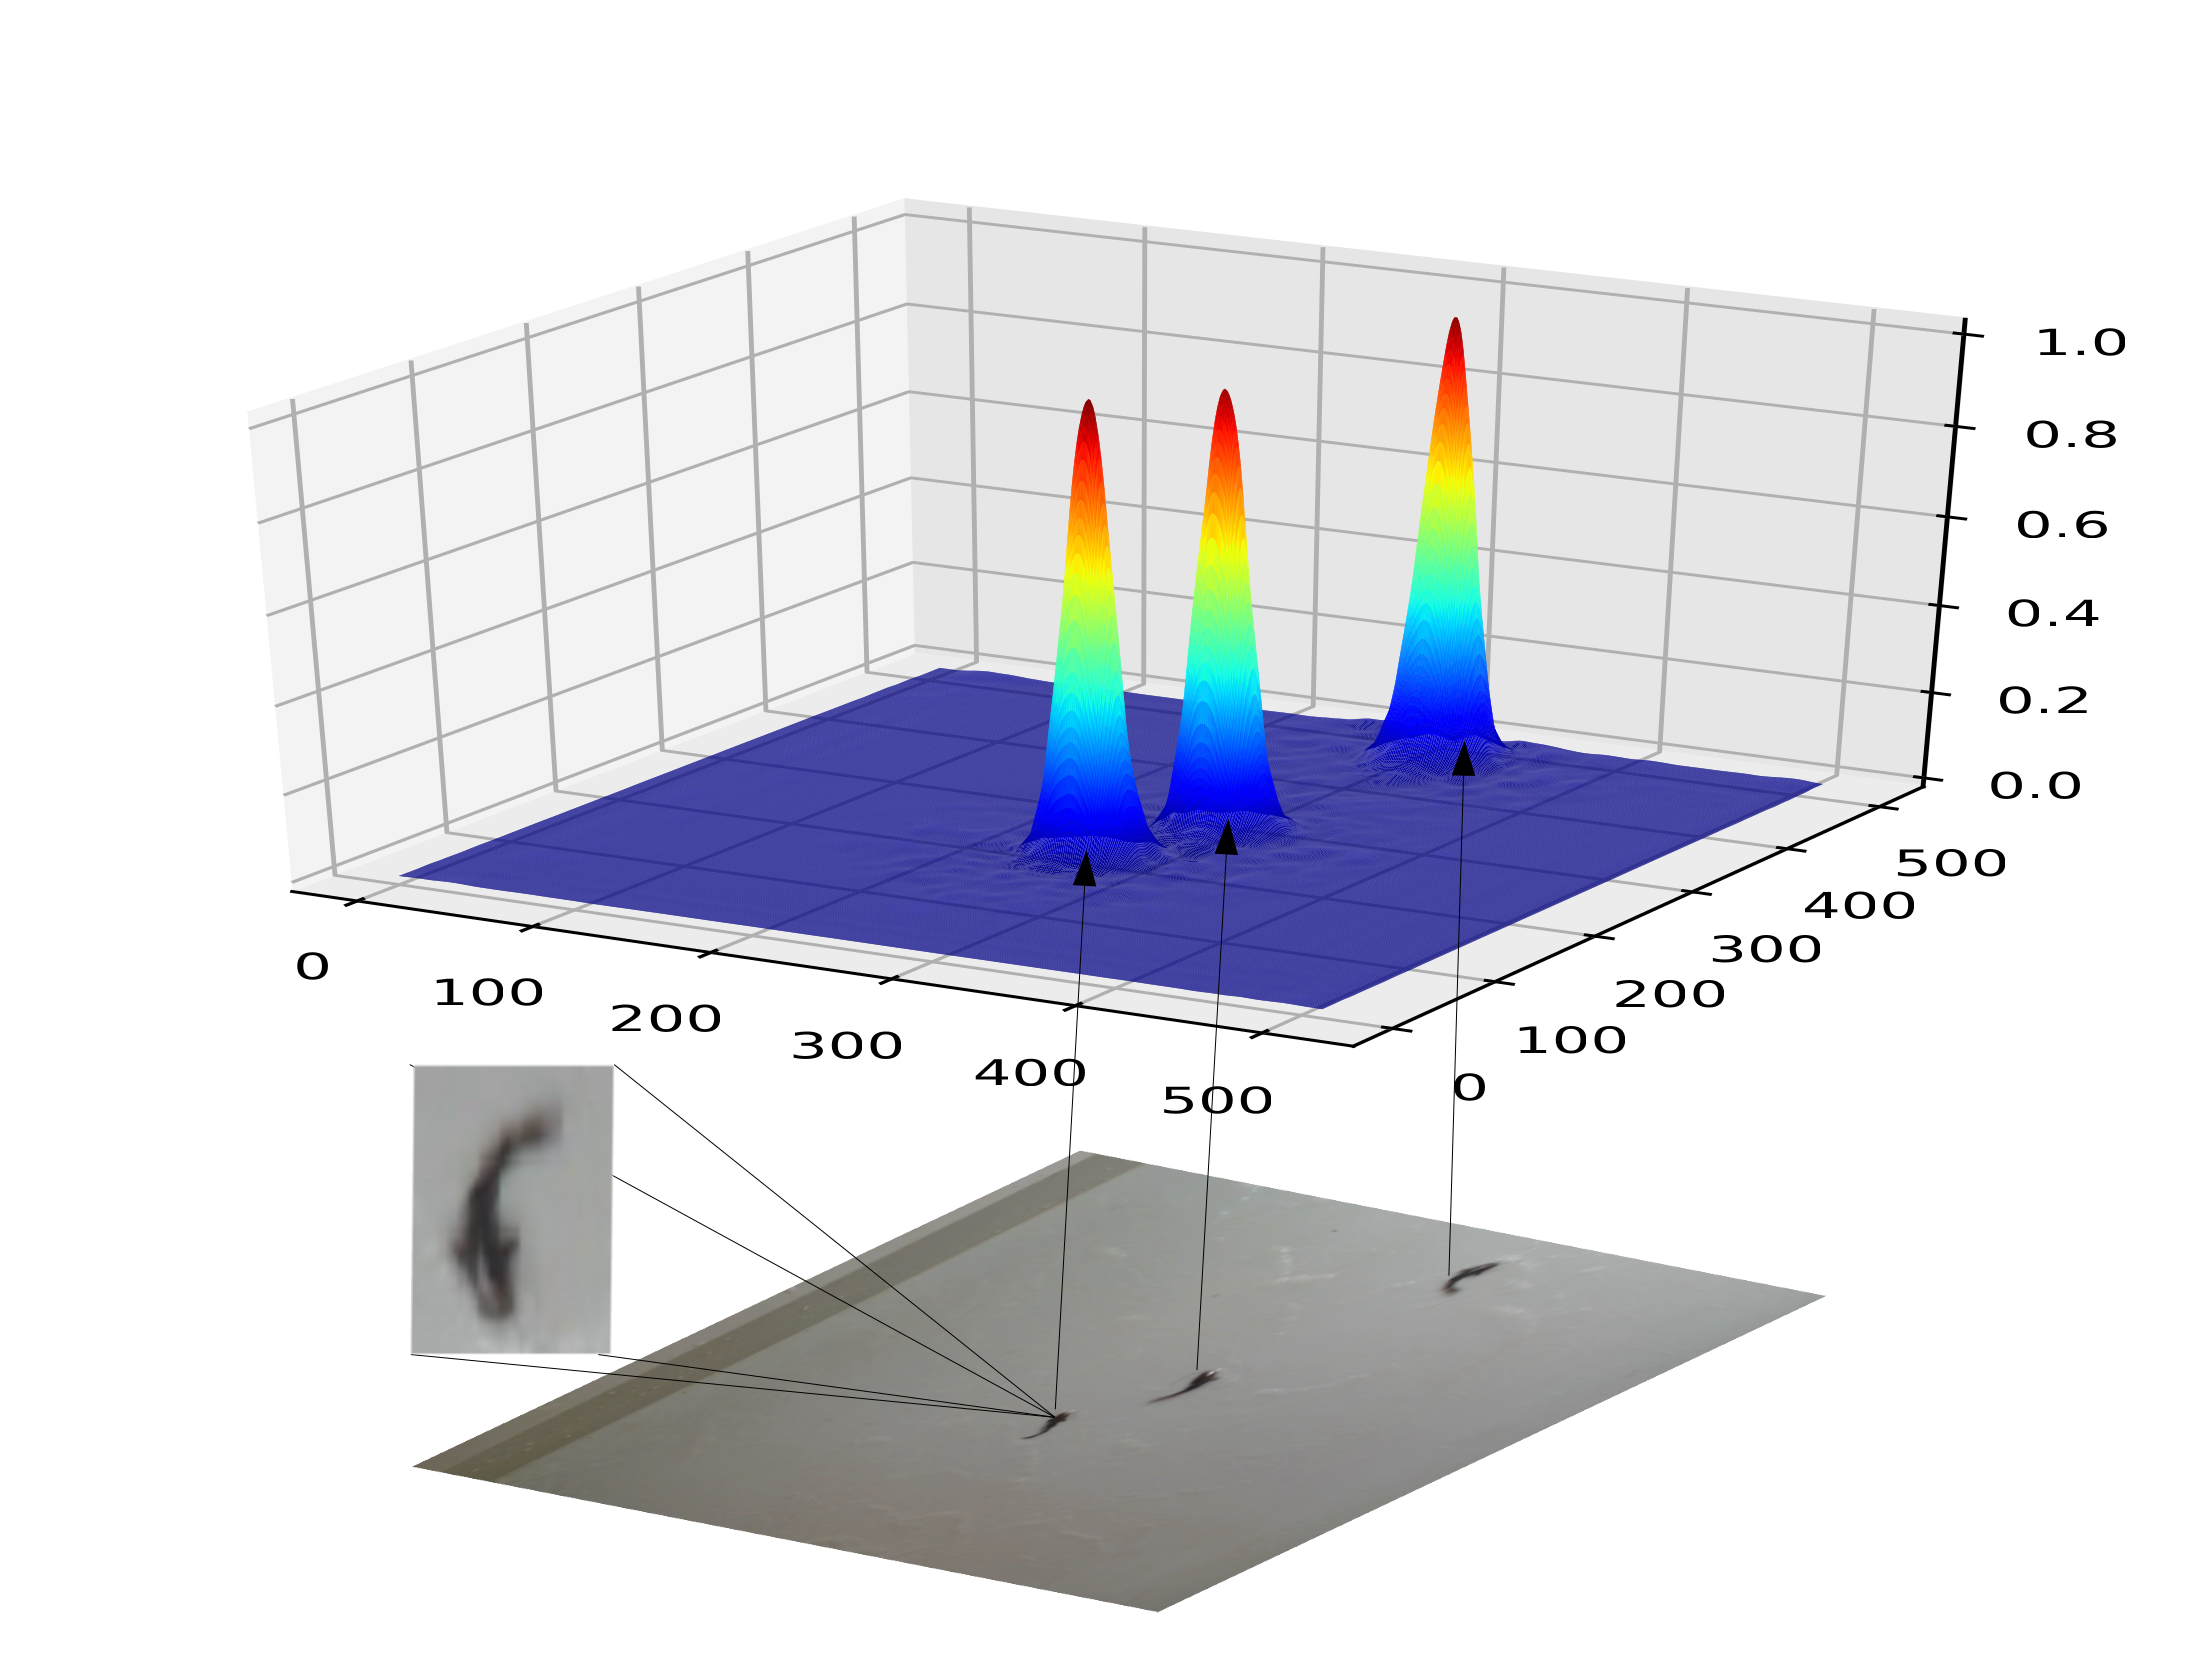
\includegraphics[width=0.9\textwidth]{image/VID06_frame000147.png}
	\caption{Ilustração do \textit{Heatmap} obtido do \textit{frame} 147 do vídeo número 6, predito pelo modelo treinado por 100 épocas.}
	\label{heatmap}
    \end{figure}

Podemos observar nas imagens da Figura \ref{fig:resultadosQuali} o quadro original, o mapa de densidade, as detecções e a avaliação da métrica \textit{F1} e a estimativa dos vetores de deslocamento.
Todos os peixes presente no quadro foram detectados e os vetores foram estimatidos para as posições anteriores. Neste caso em específico temos dois peixes próximos que foram detectados e contabilizados individualmente.

Haja vista a Seção \ref{subsec:ResultadosQ} os quadros onde a quantidade de alevinos é $\leq 6$, os alevinos são facilmente detectados. Quando a presença de peixes é $\geq 6$ a CNN detecta os alevinos em sua grande maioria, mas existe aqueles que por algum motivo tiveram uma deformação em sua forma na imagem. O movimento realizado pelo peixe diz muito sobre a sua forma.

\begin{figure}[!hbt]
	
	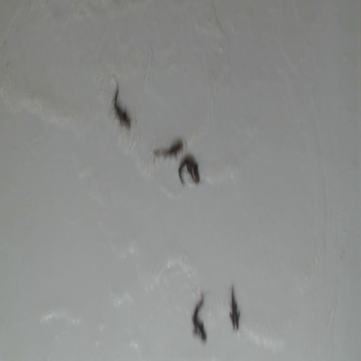
\includegraphics[width=0.4\textwidth]{image/ResultadosQ/VID09_frame000039.png}
	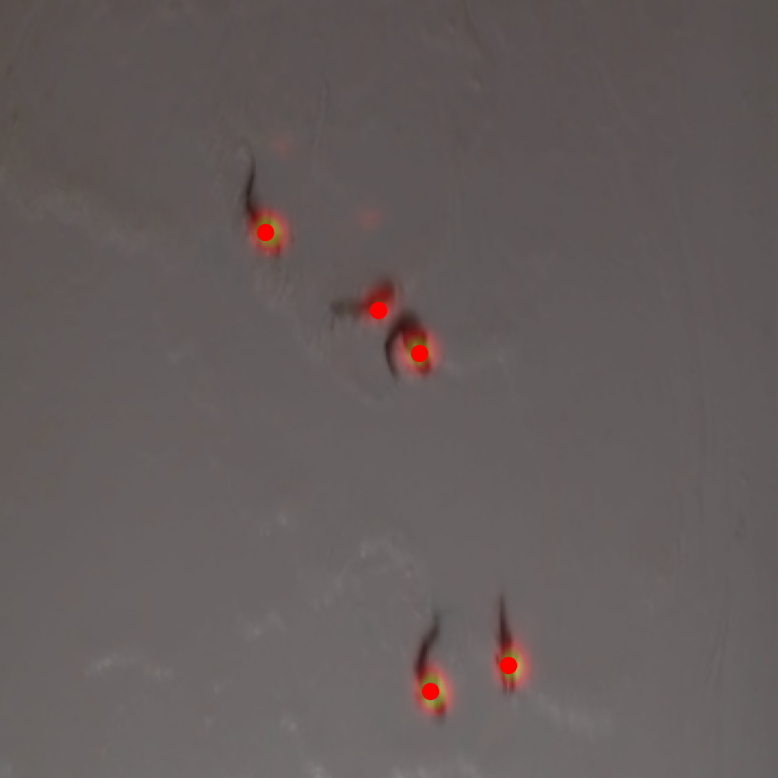
\includegraphics[width=0.4\textwidth]{image/ResultadosQ/VID09_frame000039_points_.png}
	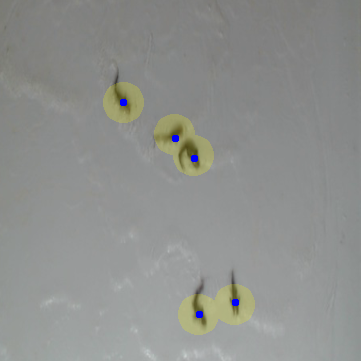
\includegraphics[width=0.4\textwidth]{image/ResultadosQ/VID09_frame000039_points.png}
	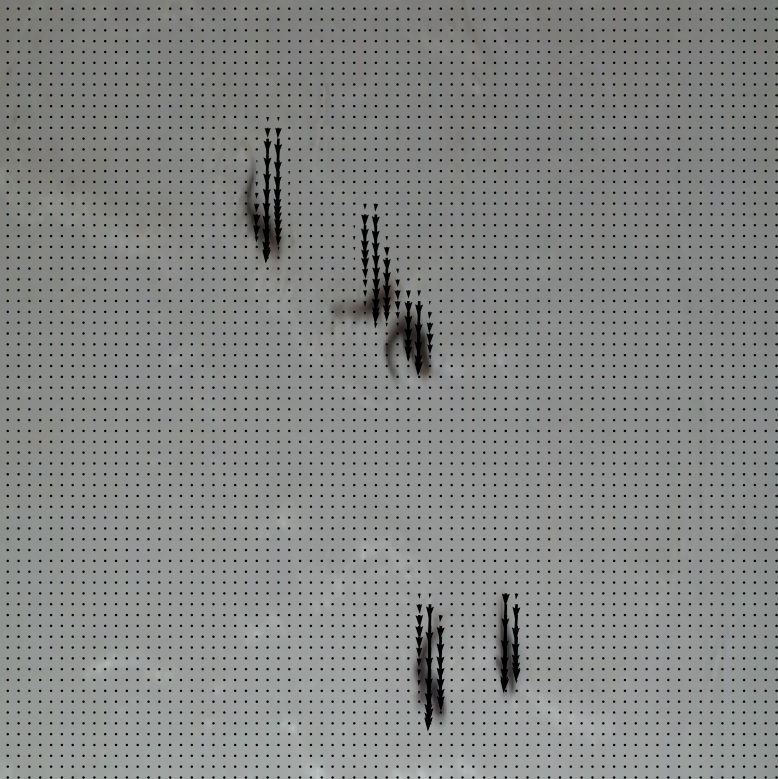
\includegraphics[width=0.4\textwidth]{image/ResultadosQ/VID09_frame000039_vectors.png}

	\caption{\label{fig:resultadosQuali} Exemplos dos resultados visuais obtidos para o quadro 30 do vídeo 09. A Figura (a) mostra a imagem original, (b) o mapa de densidade, (c) as predições e (d) a estimação dos vetores.
	}
\end{figure}

Um dos problemas da abordagem proposta esta na detecção correta do alevino quando parte do seu corpo está oclusa na imagem. Isso acontece, pois uma das características da CNN é buscar identificar o alevino considerando uma distribuição de probabilidade de um alevino estar em um pixel. Dessa forma, para que a CNN consiga predizer um alevino, boa parte do formato dele deve aparecer na imagem, para que uma resposta alta a esse padrão seja encontrada.


Nas imagens presentes na Figura \ref{fig:resultadosJuntos} temos um quadro onde existem três alevinos, porém os dois mais próximos, foram contabilizados apenas como um. Um alevino encontra-se extremamente próximo ao outro, impossibilitando de serem distinguidos a olho nu.
Em alguns quadros na sequência temos que os dois peixes chegam a se separar, porém existem casos em que dois alevinos se movem uniformemente. Essa aproximação confundi a estimativa de vetores, que estima um número de vetores deslocamento diferente.

\begin{figure}[!htb]
	
	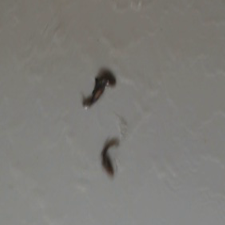
\includegraphics[width=0.35\textwidth]{image/ResultadosQ2/VID11_frame000217.png}
	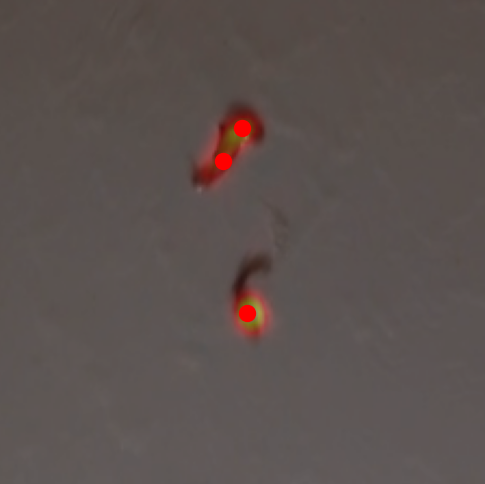
\includegraphics[width=0.35\textwidth]{image/ResultadosQ2/VID11_frame000217_points_gt_.png}
	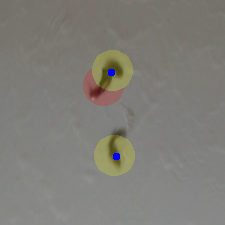
\includegraphics[width=0.35\textwidth]{image/ResultadosQ2/VID11_frame000217_points.png}
	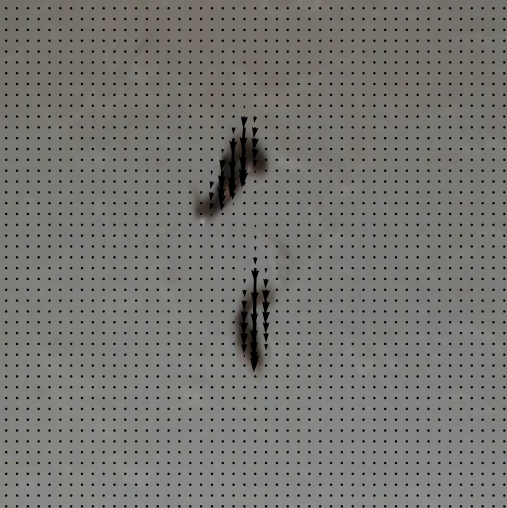
\includegraphics[width=0.35\textwidth]{image/ResultadosQ2/VID11_frame000217_vectors.png}

	\caption{\label{fig:resultadosJuntos} Exemplos dos resultados visuais obtidos para o quadro 270 do vídeo 11. A Figura (a) nos mostra a imagem original, (b) o mapa de densidade, (c) as predições e (d) a estimação dos vetores.
	}

\end{figure}



Por outro lado, outro grande desafio é detectar corretamente o formato do alevino na imagem. Podemos observar que quase sempre por conta da colisão entre eles os alevinos formam um padrão disforme ao usual.
Apesar desses desafios, o método proposto é capaz de detectar corretamente a grande maioria dos alevinos.


